\%
%%%%%%%%%%%%%%%%%%%%%%%%%%%%%%%%%%%%%%%%%%%%%%%%%%%%%%%%%%%%%%%%%%%%%%%%%%%%%%%
% Itroduccion
%%%%%%%%%%%%%%%%%%%%%%%%%%%%%%%%%%%%%%%%%%%%%%%%%%%%%%%%%%%%%%%%%%%%%%%%%%%%%%%
%
\chapter{Introduction}


%------------------------------------------------------------------------
\section{Identification of $b$-jets from gluon splitting}\label{sec:introduction}
%------------------------------------------------------------------------


The ability to identify jets containing $B$-hadrons is important for the high-\pt\ physics program of the ATLAS experiment. Two robust $b$-tagging algorithms taking
advantage of either the impact parameter of tracks~\cite{ATLAS-CONF-2010-091} or the reconstruction of secondary vertices~\cite{ATLAS-CONF-2010-042} were developped and successfully used for several analyses of the 2010 and 2011 data. Building on this experience, more advanced and performing $b$-tagging algorithms have been recently commissioned with 2011 data~\cite{ATLAS-CONF-2011-102}.
All $b$-tagging algorithms rely on the relatively long decay length of $B$-hadrons that gives rise to large impact parameter children tracks and displaced decay secondary vertices. The more advanced taggers %are based on Monte Carlo predictions for the signal ($b$-jet) or background (light- or $c$-jet) hypotheses and
use multivariate techniques %such as likelihood ratios and neural networks 
to further increase the discrimination between $b$-jets and light jets.
These algorithms, however, are not sensitive to the number of $B$-hadrons within the jet. In particular they would equally tag gluon jets if they give rise to a close-by $B$-hadron pair via gluon splitting, as depicted in Fig.~\ref{fig:gbbcartoon}. We will henceforth call ``merged'' $b$-jets or $b \bar{b}$ jets the $b$-tagged jets containing two $B$-hadrons. The ability to single out $b$-tagged jets from gluon splitting has several applications in different lines of analysis: measurement of QCD beauty production, $t\bar{t}$ and single top production, reduction of background in searches with $b$-quarks in the final state, and the study of substructure in fat jets, where $g\rightarrow b\bar{b}$ jets compete with boosted $Z\rightarrow b\bar{b}$ and $H\rightarrow b\bar{b}$ jets.
\begin{figure}[h]
\centering
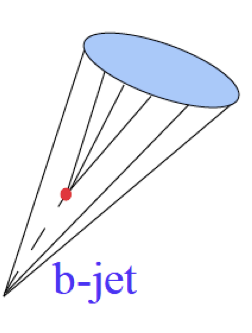
\includegraphics[width=0.25\textwidth]{FIGS/Single_b.png}
\hspace{1cm}
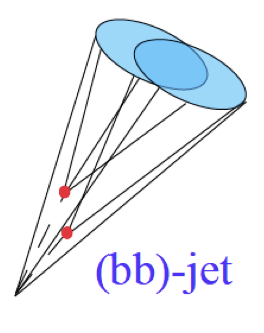
\includegraphics[width=0.25\textwidth]{FIGS/Merged_bb.png}
  \caption{$b$-tagging algorithms select jets originating both from the fragmentation of a single $b$ quark (``single'' $b$-jets, left image) or from the splitting of a gluon into a pair of close-by $b \bar{b}$ quarks (``merged'' $b$-jets, right image).}
  \label{fig:gbbcartoon}
\end{figure}

%This note presents a method that allows the separation of merged and single $b$-jets with a multivariate analysis that exploits their substructure differences.
There are two possible strategies to attempt the identification of $b$-jets containing two $B$-hadrons. One of them relies on the direct reconstruction of the two $B$-decay secondary vertices~\cite{CDFAzimutalCorrelation}. This has the further advantage of allowing the measurement of the angular separation between the $B$-hadrons, but suffers from the low efficiency of a double $b$-tag requirement plus additional reconstruction inefficiencies at small angular separation between the two $B$s. In this paper we develop an alternative method that does not rely on explicitly finding vertices, but exploits the substructure differences between single and merged $b$-jets, combining them in a multivariate analysis. 

The note is organized as follows. In section~\ref{sec:motivation} we review the physics cases where this tool finds natural applications. Sections~\ref{sec:Simulation} and~\ref{sec:ObjSelection} review the Data and Monte Carlo samples and their reconstruction and section~\ref{sec:EventSelection}, the criteria for selection of events, jets and tracks. The kinematic variables that differentiate between single and merged $b$-jets are discussed in section~\ref{sec:kinematic} and the validation of their MC distributions with QCD data in section~\ref{sec:validation}.  The construction of the multi-variate discriminator is presented in section~\ref{sec:likelihood_tagger} and the discussion of the systematic uncertainties in section~\ref{sec:systematics}. Section~\ref{sec:otherMC} investigates the performance of the tagger with other Monte Carlo generators and, finally, section~\ref{sec:Conclusions} summarizes the results and discusses future improvements and new ideas. %lines of action.
% Section~\ref{sec:Detector} describes the ATLAS calorimeters and tracking system. Sections~\ref{sec:EventSelection} and \ref{sec:Simulation} describe the event selection and Monte Carlo simulation used. Section~\ref{sec:ObjSelection} describes the way in which jets are reconstructed. Sections~\ref{sec:Strategy} and~\ref{sec:Determination} describe the strategy of the method and the procedure used to derive the Response correction. The improvement achieved in jet fractional resolution and the reduction on the dependance of the jet flavor sample composition are shown in Sections~\ref{sec:Results_improvement_mc},~\ref{sec:Results_improvement_data} and~\ref{sec:Results_flavor}. Finally, results for other calibrations are presented in~\ref{app:appendix_d} and ~\ref{app:appendix_c}


%------------------------------------------------------------------------
\section{Physics Motivation}\label{sec:motivation}
%------------------------------------------------------------------------


Within the Standard Model (SM) a range of production channels exist for
heavy-quark jets, \eg pure QCD production or in association with heavy bosons
($W, Z, H$). Furthermore, $b$-quarks enter in many collider searches, notably
because they are produced in the decays of various SM particles, \eg top
quarks and the Higgs boson (if light), and of numerous particles appearing
in proposed extensions of the SM. The ability to distinguish genuine $b$-quark jets from those produced via gluon splitting is thus of wide application. Here we briefly discuss three cases, the measurement of QCD $b$ quark production, the reduction of background in SM and BSM analyses with $b$ quarks in the final state, and studies of jet substructure.%
%
\\[5mm]
{\em The measurement of the inclusive $b$-jet spectrum}
\\[5mm]
The simplest and most fundamental measurement of heavy-quark jet production is
the inclusive heavy-quark jet spectrum, which is dominated by pure QCD
contributions.  Studies of QCD bottom jets production are of intrinsic interest
because of the correspondence between parton level production and the observed
hadron level, and their potential to provide information on the $b$-quark
parton distribution function, the only component of the proton structure
thought to be generated entirely perturbatively from the DGLAP evolution of the
other flavours.  The theoretical calculation of the inclusive
$b$-jet spectrum presents the striking feature of having rather important uncertainties ($\sim 50\%$), considerably larger than the
corresponding ones for the normal (light) jet inclusive spectrum ($\sim
10$-$20\%$), see for example~\cite{Frixione:1996nh}.  

The origin of these uncertainties are reviewed in a recent paper by Banfi, Salam and Zanderighi~\cite{Salam.AccurateHQ}, from which we have taken Fig.~\ref{fig:bjets_qcd}. Its top panel shows the $K$-factor, the ratio of the next-to-leading order (NLO) to the leading order (LO) cross section, obtained with MCFM for the LHC design energy  ($pp$, $\sqrt{s}= 14$ TeV).
\begin{figure}[tp]
\centering
%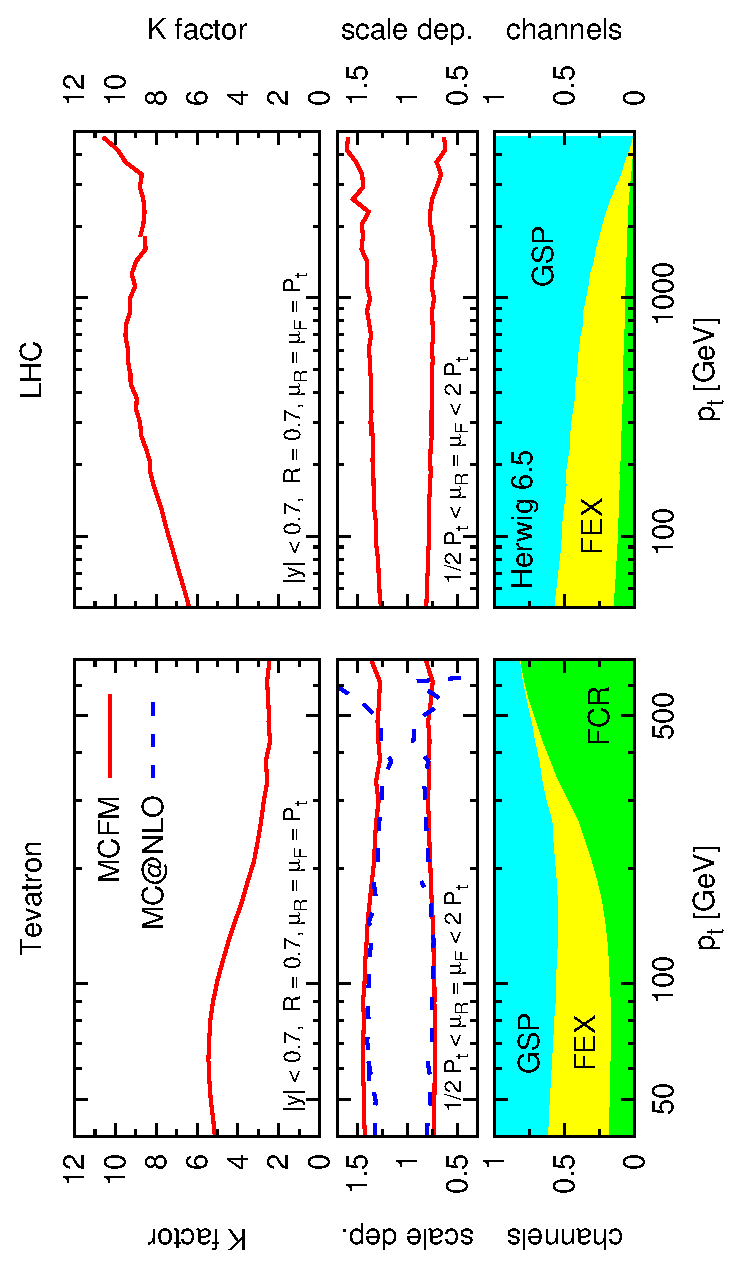
\includegraphics[height=0.7\textwidth,viewport=20 305 340 590,clip,angle=270]{FIGS/bjets_qcd.eps}
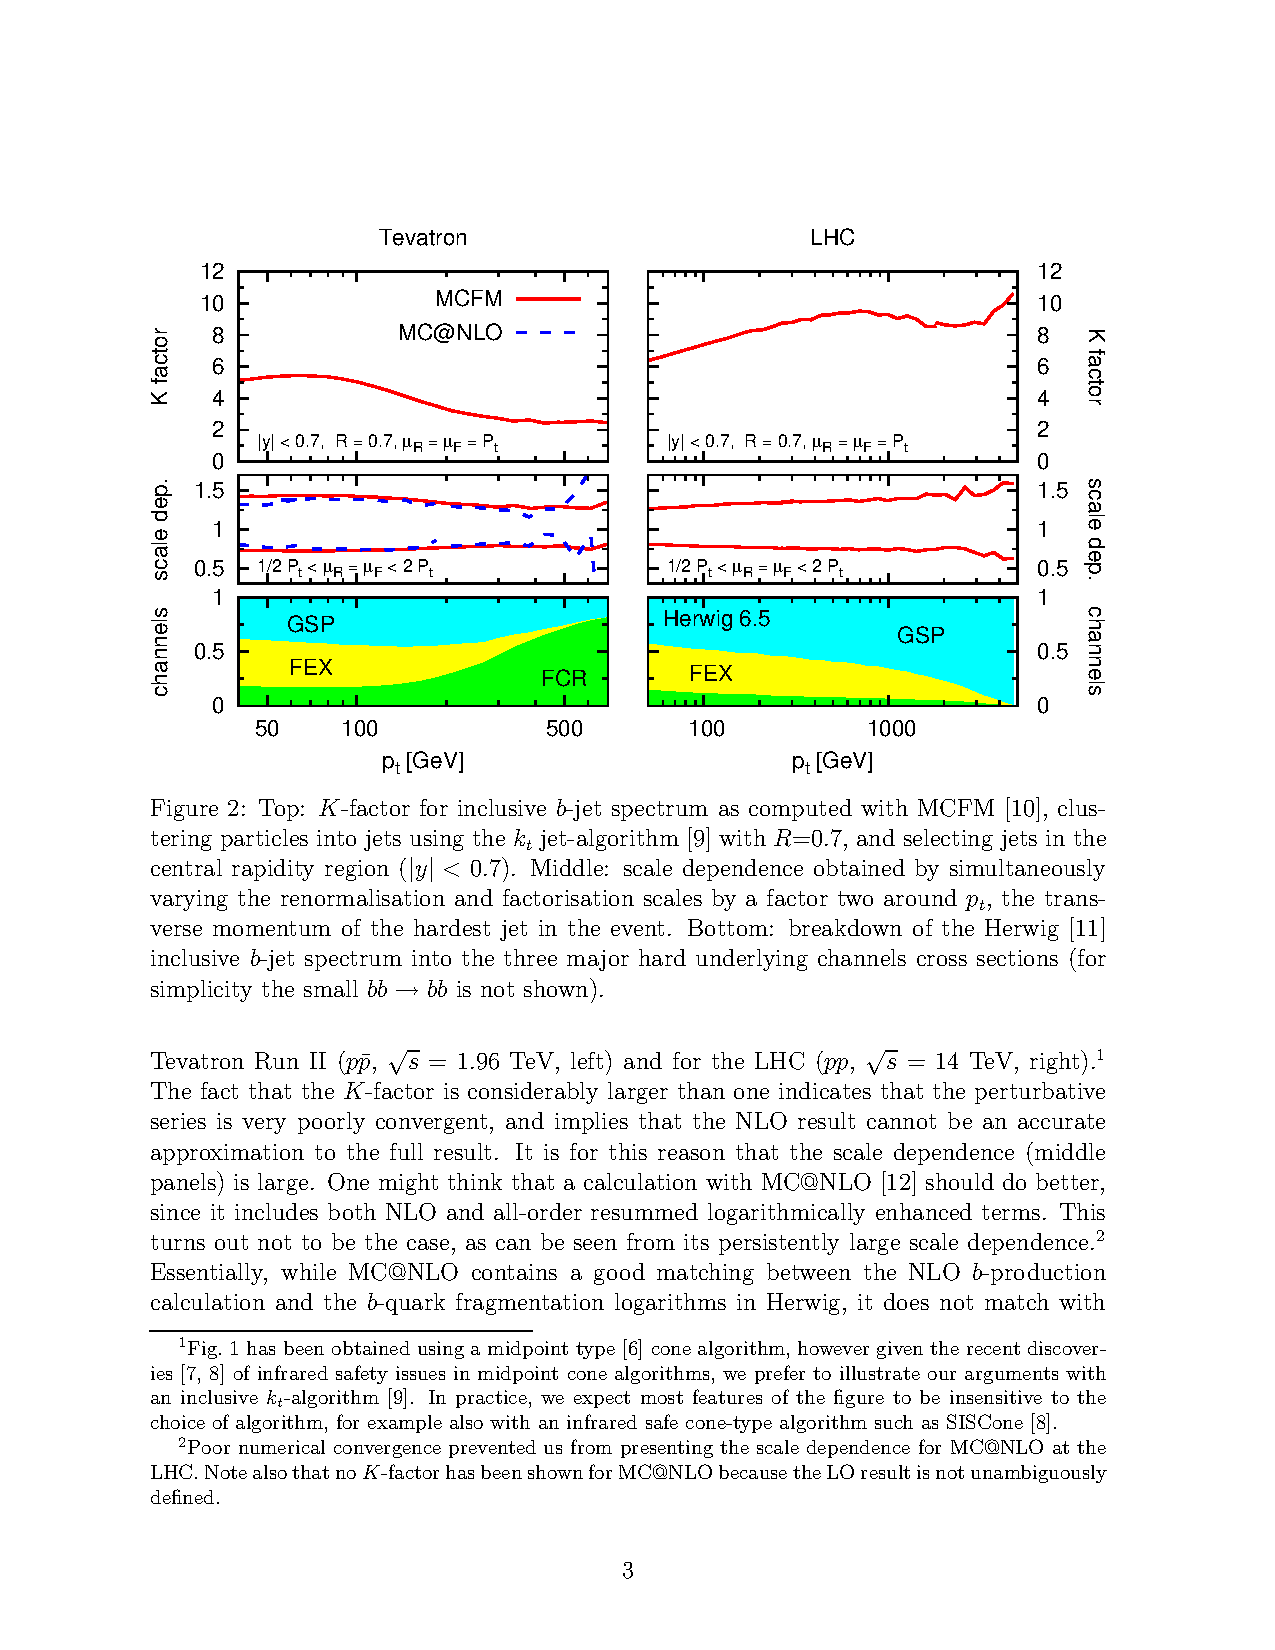
\includegraphics[height=0.7\textwidth,viewport=300 410 530 690,clip]{FIGS/bjets_qcd.pdf}
  \caption{Top: $K$-factor for inclusive $b$-jet spectrum taken
  from~\cite{Salam.AccurateHQ}, clustering particles into jets using the $k_t$
  jet-algorithm~\cite{kt1}  with $R$=0.7, and selecting jets in the central
  rapidity region ($|y| <0.7$). Middle: scale dependence obtained by
  simultaneously varying the renormalisation and factorisation scales by a factor
  two around $\pt$, the transverse momentum of the hardest jet in the event.
  Bottom: breakdown of the Herwig \cite{Herwig} inclusive $b$-jet spectrum into
  the three major underlying channels, flavor creation (FCR) flavor excitation
  (FEX) and gluon splitting (GSP).}
  \label{fig:bjets_qcd}
\end{figure}
The fact that NLO terms are considerably larger than the LO ones indicates
that the perturbative series is very poorly convergent, and implies that the
NLO result cannot be an accurate approximation to the full result.
It is for this reason that the scale dependence (middle panels) is large.  The
poor convergence of the perturbative series is related to the different
channels for heavy quark production. At leading order only the so-called
flavour creation channel (FCR) is present, $\ell \ell \to b\bb$, where $\ell$
is a generic light parton (quark or gluon), see fig.~\ref{fig:qcd_diagrams}.
\begin{figure}[tp]
\centering
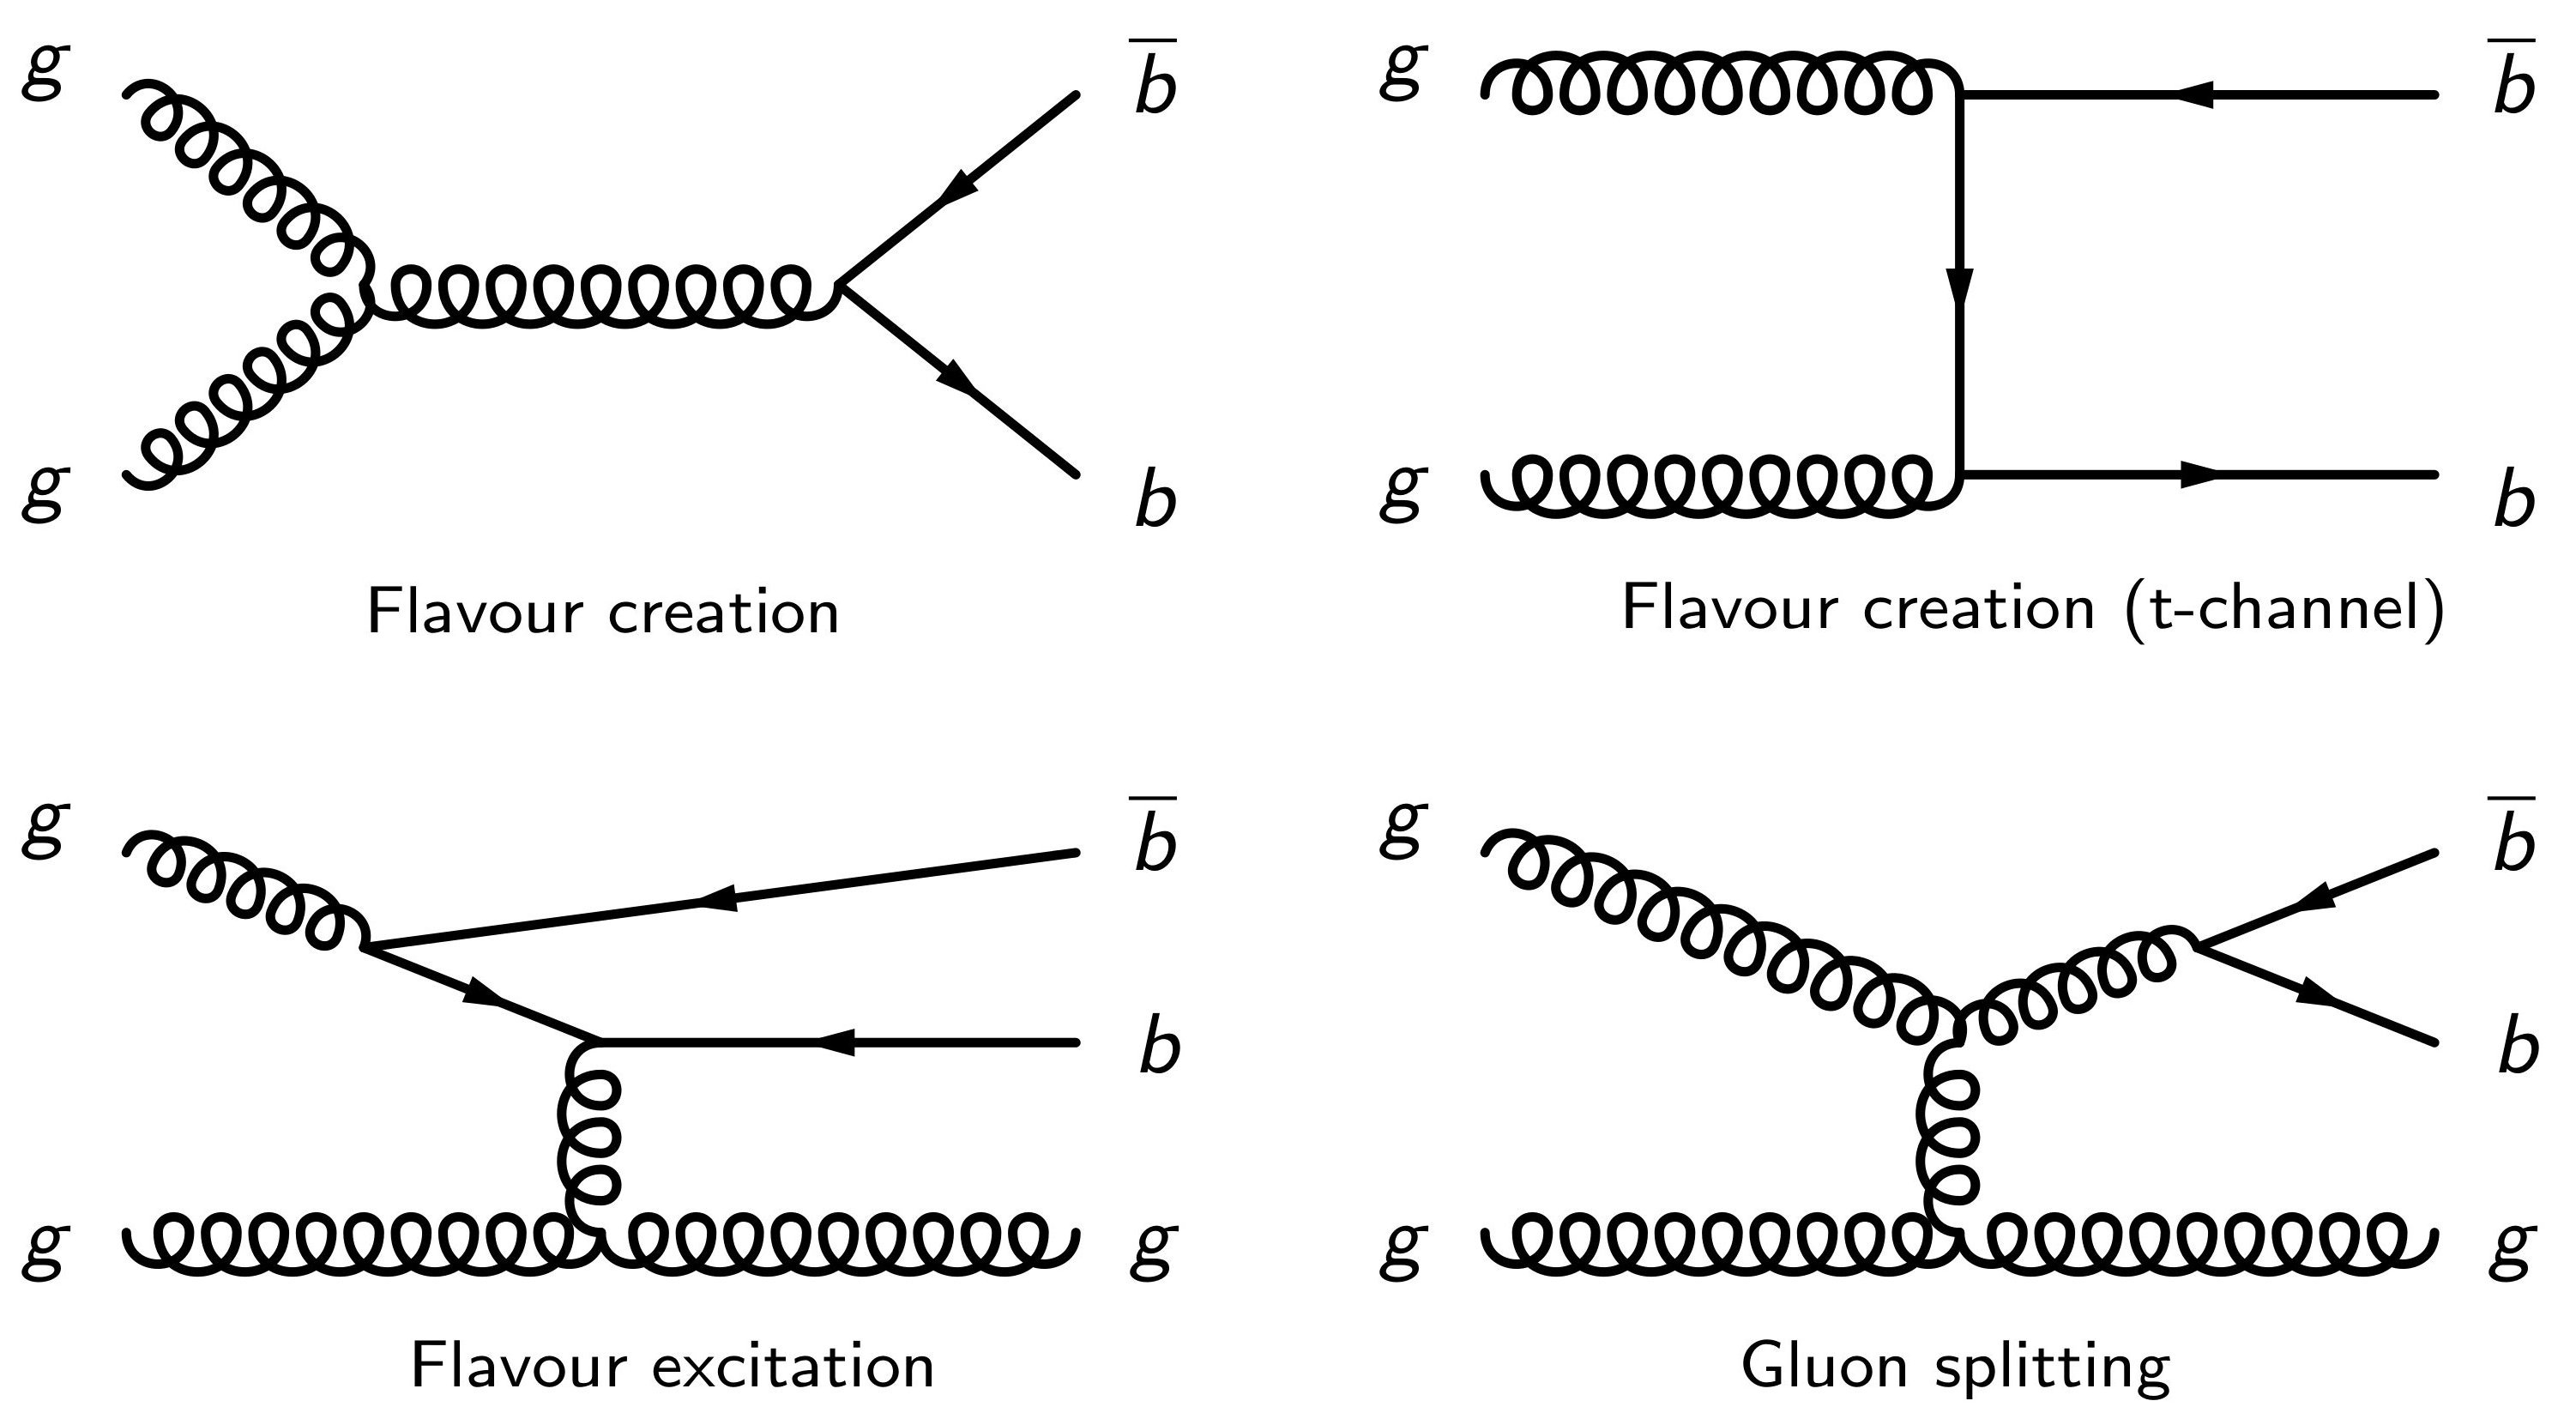
\includegraphics[width=0.8\textwidth]{FIGS/bb_diagrams.jpg}
\caption{Typical Feynman diagrams for the 3 processes contributing up to next-to-leading order to QCD bottom production: (a-b) Flavor creation (FCR), (c) Flavor excitation (FEX), (d) Gluon splitting (GSP).}
  \label{fig:qcd_diagrams}
\end{figure}
At NLO, two new channels open up, often referred to as flavour excitation (FEX) and gluon splitting (GSP). In the former, a gluon from one of the incoming hadrons splits collinearly into a $b \bar{b}$-pair and one of those $b$-quarks enters the hard $b\ell \to b\ell$ scattering. In the gluon splitting process, the hard scattering LO diagram is of the form $\ell \ell \to \ell \ell$, and one of the final-state light partons (at NLO always a gluon) splits collinearly into a $b \bar{b}$-pair that the clustering algorithm can classify within the same jet. A jet containing both $b$ and $ \bar{b}$ is considered to be just a $b$-jet in standard definitions.
The various channels can be conveniently separated with a parton shower Monte Carlo generator such as Herwig~\cite{Herwig}, where one can determine the underlying hard channel from the hard process in the event record. Their relative contributions to the total $b$-jet spectrum are shown in the bottom panel of fig.~\ref{fig:bjets_qcd}.  One sees that the supposedly LO channel (FCR) is nearly always smaller than the two channels that enter only at NLO (FEX and GSP). %\footnote{This is because both NLO channels receive a strong enhancement from collinear logarithms, going as $\as^2 (\as \ln(\pt/\Mb))^n$ for flavour excitation~\cite{DGLAP} and $\as^2 \cdot \as^n \ln^{2n-1}(\pt/\Mb)$ for gluon splitting ($n\ge 1$)~\cite{bmult}}.

The largest residual uncertainties are associated with the channel with the
most logarithms, gluon splitting. This channel however does not even correspond
to one's physical idea of a $b$-jet, \ie the one induced by a hard $b$-quark, and it
seems somehow unnatural to include it at all as part of one's $b$-jet spectrum.
Reference~\cite{Salam.AccurateHQ} thus proposes a new approach to improving the accuracy of the prediction of
the $b$-jet spectrum, where $b$-jets definition maintains the correspondence
between partonic flavour and jet flavour. Specifically, a jet containing equal
number of $b$-quarks and $b$-antiquarks is considered to be a light jet, so
that jets identified as gluon splitting are removed from the $b$-jet spectrum. %
%
\\[5mm]
{\em Rejection of background in SM analyses and beyond-SM searches}
\\[5mm]
Efficient tagging of merged $b$-jets from gluon splitting can provide an important handle to understand, estimate and/or reject $b$-tag backgrounds to Standard Model and new physics searches at the LHC.

Standard Model physics analyses that rely on the presence of $b$ quarks in the final state such as top quark physics, either in the $t\bar{t}$ or the single top channels, and associated
Higgs production: $WH\rightarrow\ell\nu b\bar{b}$ and $ZH\rightarrow\nu\nu
b\bar{b}$, suffer from reducible backgrounds from QCD (that can produce $b$-jets from gluon splitting) and, most importantly, from the irreducible background due to  
$W$ bosons produced in association with $b$ quarks.  Fig.~\ref{fig:Wplusb} shows
the two leading order processes that give rise to $W$ bosons with at least one
$b$-jet. In the first process, which can be thought of as a higher order correction to $W$ + jets production, the $b$ quark pair is produced at small angles by gluon
splitting and can often be reconstructed as a merged jet.
\begin{figure}[hp]
\centering
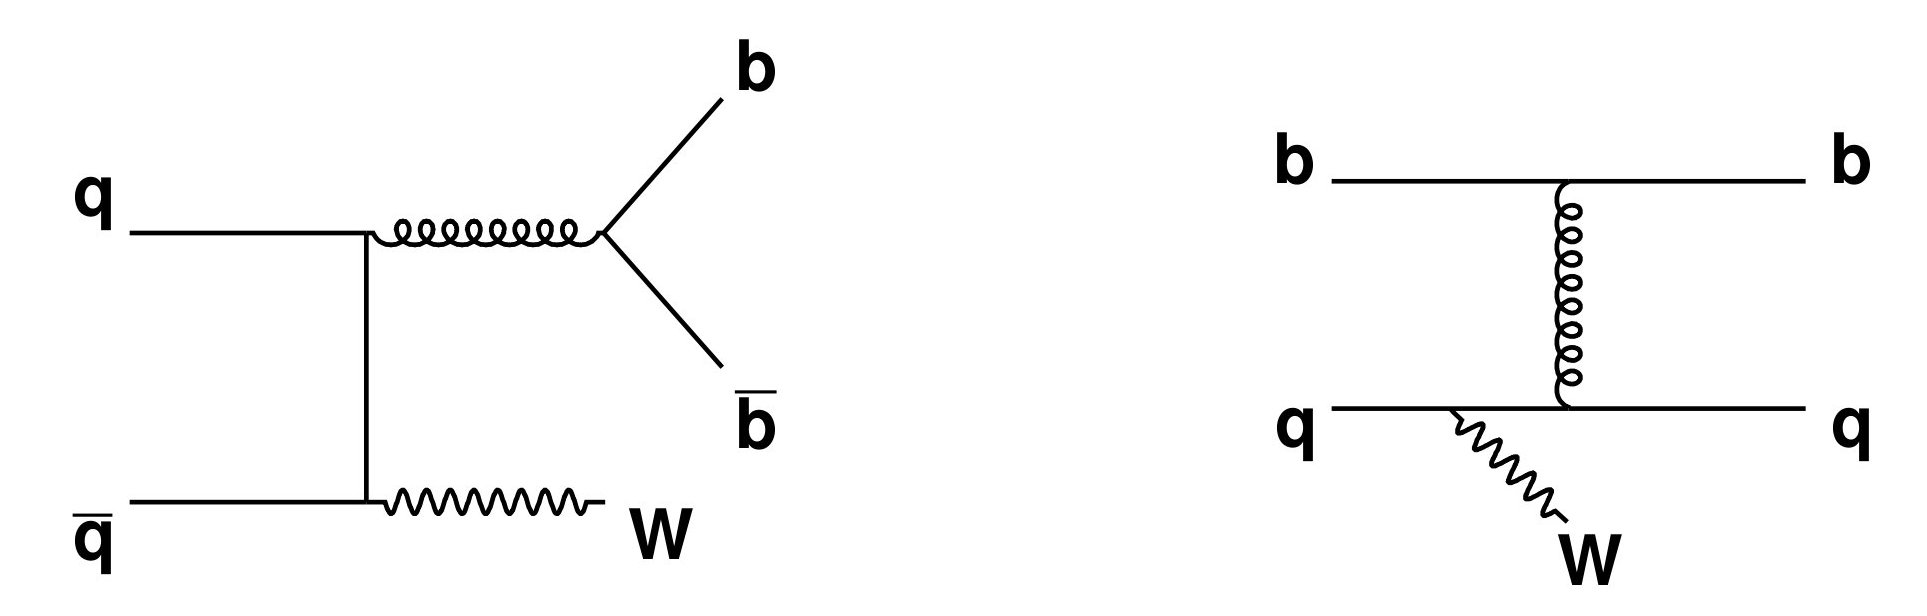
\includegraphics[width=0.6\textwidth]{FIGS/Wbb_diagram.jpg}
\caption{Leading order Feynman diagrams for $W$ production in association with $b$ quarks.}
\label{fig:Wplusb}
\end{figure}
NLO calculations of the production of $W$ bosons and two jets with at least one $b$ quark at the LHC for jet $\pt > 25$ GeV, and $|\eta| < 2.5$~\cite{Campbell:2006} indicate that the cross section for $W(b\bar{b})j$ is almost a factor of two higher than $Wb\bar{b}$, and about a third of $Wbj$, where  $W(b\bar{b})j$ denotes the case in which the two $b$ quarks are merged into the same jet. 

New physics searches with $b$ quarks in the final state can also greatly benefit from rejection of QCD and $W+b$ backgrounds with $b$-jets arising from gluon splitting. For example consider the search for supersymmetry in the \met\ + $b$-jets channel~\cite{ATLAS-CONF-2011-098}. Within the framework of a generic $R$-parity conserving minimal supersymmetric extension of the SM The coloured superpartners of quarks and gluons, the squarks and gluinos, are expected to be copiously produced via the strong interaction at the LHC. The
partners of the right-handed and left-handed quarks, qR and qL, can mix to form two mass eigenstates, and these mixing effects being proportional to the corresponding fermion masses, they are expected to become most important for the third generation to yield sbottom ($b_1$ ) and stop ($t_1$ ) mass eigenstates significantly lighter than other squarks. Both sbottom and stop chain decay to $b$ quarks and the lightest supersymmetric particle, producing the expected signal of \met\ + $b$-jets. 
%
%
\\[5mm]
{\em Jet substructure and boosted objects}
\\[5mm]
At the LHC, many of the particles considered to be heavy at previous accelerators will be frequently produced with a transverse momentum greatly exceeding their rest mass. Good examples are the electro-weak gauge bosons $W^\pm$ and $Z^0$, the top quark, the Higgs boson or bosons and possibly other new particles in the same mass range. These boosted objects, produced either because they recoil against other energetic objects or because they arise from decays of even heavier BSM particles, can form upon decay a highly collimated topology too close to be resolved by a jet algorithm. For theses cases, sophisticated tools have been developed in the last years~\cite{boost2010,boost2010b} to analyse the substructure of the ensuing jet and reveal its heavy-particle origin. 

The study of $b\bar{b}$ jets from gluon splitting is an ideal testbed for studying jet substructure in data, as it provides a large supply of boosted, merged jets. Furthermore, understanding $g\rightarrow b \bar{b}$ jets is important as they are themselves the background to boosted object searches, like $Z\rightarrow b\bar{b}$ or $H\rightarrow b \bar{b}$.  In particular, it has recently been suggested~\cite{Butterworth:2008iy} that $WH$ and $ZH$ production become potential discovery and analysis channels by restricting one’s attention to the $\sim5$\% of events in which the vector and Higgs bosons have large transverse momentum, ${\pt}_H\gtrsim200$ GeV. Understanding the much more common QCD events with merged $b\bar{b}$ jets will be essential before attempting to measure these rare final states.





